%% Begin slides template file
\documentclass[11pt,t,usepdftitle=false,aspectratio=169]{beamer}
%% ------------------------------------------------------------------
%% - aspectratio=43: Set paper aspect ratio to 4:3.
%% - aspectratio=169: Set paper aspect ratio to 16:9.
%% ------------------------------------------------------------------

%% Graphics
\usepackage{graphicx}
\usepackage{tikz}
\usepackage{rotating}

\usepackage{media9} 

\usepackage{xcolor}
\usepackage{xfrac}
\usepackage[export]{adjustbox}[2011/08/13]

\usepackage{booktabs}

%% Tables and Lists
\usepackage{enumerate}
\usepackage{multicol}
\usepackage{geometry}
\usepackage{tabu}
\usepackage{listings}
\usepackage{tabularx}
\usepackage{siunitx}

\usepackage{float} 
\usepackage{svg}
\usepackage{subcaption}

%% special packages
\usepackage{caption}
\captionsetup[figure]{font=tiny,labelfont=tiny}
\usepackage{multimedia}

\usepackage{animate}

\usetheme[nototalframenumber,logo]{uibk} % nototalframenumber,foot, also an option
%% ------------------------------------------------------------------
%% - foot: Add a footer line for conference name and date.
%% - logo: Add the university logo in the footer (only if 'foot' set).
%% - bigfoot/sasquatch: Larger font size in footer.
%% - nototalslidenumber: Hide the total number of slides (only if 'foot' set)
%% - license: Add CC-BY license symbol to title slide (e.g., for conference uploads)
%%   (TODO: At the moment no other licenses are supported.)
%% - licenseall: Add CC-BY license symbol to all subsequent slides slides
%% - url: use \url{} rather than \href{} on the title page
%% ------------------------------------------------------------------

%% ------------------------------------------------------------------
%% The official corporate colors of the university are predefined and
%% can be used for e.g., highlighting something. Simply use
%% \color{uibkorange} or \begin{color}{uibkorange} ... \end{color}
%% Defined colors are:
%% - uibkblue, uibkbluel, uibkorange, uibkorangel, uibkgray, uibkgraym, uibkgrayl
%% The frametitle color can be easily adjusted e.g., to black with
%% \setbeamercolor{titlelike}{fg=black}
%% ------------------------------------------------------------------

%\setbeamercolor{verbcolor}{fg=uibkorange}
%% ------------------------------------------------------------------
%% Setting a highlight color for verbatim output such as from
%% the commands \pkg, \email, \file, \dataset 
%% ------------------------------------------------------------------


%% information for the title page ('short title' is the pdf-title that is shown in viewer's titlebar)
\title[Vicsek Model]{Vicsek Model}
\subtitle{A 2D model for modelling swarm behaviour}
\URL{}

\author[Florian Kluibenschedl, René Schwarz, Ariel Harnik]{Florian KLUIBENSCHEDL, René SCHWARZ and Ariel HARNIK}
%('short author' is the pdf-metadata Author)
%% If multiple authors are required and the font size is too large you
%% can overrule the font size of author and url by calling:
%\setbeamerfont{author}{size*={10pt}{10pt},series=\mdseries}
%\setbeamerfont{url}{size*={10pt}{10pt},series=\mdseries}
%\URL{}
%\subtitle{}

\footertext{Experiment 4}
\date{2021-11-08}

\headerimage{3}
%% ------------------------------------------------------------------
%% The theme offers four different header images based on the
%% corporate design of the university of innsbruck. Currently
%% 1, 2, 3 and 4 is allowed as input to \headerimage{...}. Default
%% or fallback is '1'.
%% ------------------------------------------------------------------

\begin{document}

%% ALTERNATIVE TITLEPAGE
%% The next block is how you add a titlepage with the 'nosectiontitlepage' option, which switches off
%% the default behavior of creating a titlepage every time a \section{} is defined.
%% Then you can use \section{} as it's originally intended, including a table of contents.
% \usebackgroundtemplate{\includegraphics[width=\paperwidth,height=\paperheight]{titlebackground.pdf}}
% \begin{frame}[plain]
%     \titlepage
% \end{frame}
% \addtocounter{framenumber}{-1}
%\usebackgroundtemplate{}}

%% Table of Contents, if wanted:
%% this requires the 'nosectiontitlepage' option and setting \section{}'s as you want them to appear here.
%% Subsections and subordinates are suppressed in the .sty at the moment, search
%% for \setbeamertemplate{subsection} and replace the empty {} with whatever you want.
%% Although it's probably too much for a presentation, maybe for a lecture.
% \begin{frame}
%     \vspace*{1cm plus 1fil}
%     \tableofcontents
%     \vspace*{0cm plus 1fil}
% \end{frame}


	%% this sets the first PDF bookmark and triggers generation of the title page
	\section{Vicsek model}

	%% this just generates PDF bookmarks
	\subsection{Content}
	%% first slide
	\begin{frame}
		\frametitle{Content}
  		\textbf{1) Motivation and Theory.} 
  		
  		\bigskip
  		\textbf{2) Periodic Boundaries.} 
  		
  		\bigskip
  		\textbf{3) Reflecting Boundaries.}
  		
  		\bigskip
  		\textbf{4) Periodic Boundaries with Vision.}
  		
  		\bigskip
  		\textbf{5) Reflecting Boundaries with Vision.}
  		
  		\bigskip
  		\textbf{6) Conclusion.} + discussion.
	\end{frame}

	\subsection{Motivation and Theory}

\begin{frame}
	\frametitle{1) Motivation and Theory}
	\textbf{Q: Why is it interesting?}
	
	Applications.\footnote{\tiny{T. Vicsek. \textit{Novel Type of Phase Transition in a System of Self-Driven Particles}. VOLUME 75. NUMBER 6. PHYSICAL REVIEW LETTERS, 1995}}$^,$\footnote{\tiny{F. Ginelli. \textit{The Physics of the Vicsek Model}. VOLUME 225. NUMBER 11–12. The European Physical Journal Special Topics, 2016}}
	\begin{itemize}
	    \item Living systems like the collective motion of birds, fish schools, bacteria colonies or cellular migrations 

	    \item Physical systems like ferromagnetism
	    
	    \item Simple model
	\end{itemize}
\end{frame}

\begin{frame}
	\frametitle{1) Motivation and Theory}
	\textbf{Q: Why is it so simple?}
	
	\begin{itemize}
	    \item Each particles direction is influenced by only it's neighboring particles within a radius $R$ 
	    
	    \item New position within one molecular dynamics step is given by equation of motion
	    	\begin{equation}
	        	\mathbf{r}_{t + \Delta t}^i = \mathbf{r}_t^i + \mathbf{v}_t^i \cdot \Delta t
	    	\end{equation} \noindent
	    with $\mathbf{v}_t^i = v \cdot \mathbf{u}_t^i$, where $v = \mathrm{const.}$ and $\mathbf{u}_t^i = \left( \begin{array}{c}
	         \cos{(\theta_t^i)}  \\
	         \sin{(\theta_t^i)}
	    \end{array} \right)$ 
	\end{itemize}
	%\begin{figure}[H]
  	%	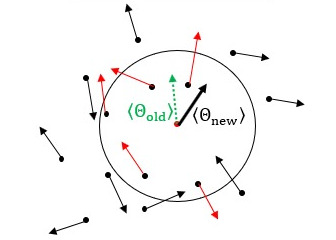
\includegraphics[width=0.3\textwidth]{images/chapter1/particle_direction.jpeg} 
  	%	\caption*{ales.airliquide. \url{https://ales.airliquide.com/our-markets/photovoltaic}. Accessed on the 15.11.2021.}
	%\end{figure}
\end{frame}

\begin{frame}
	\frametitle{1) Motivation and Theory}
	\begin{itemize}
	    \item Updating $\theta_t^i$ using the expression
	    	\begin{equation}
	        	\theta_{t + \Delta t}^i = \langle \theta_t^j \rangle_{|r_i - r_j| < R} + \sqrt{2 D_\mathrm{rot} \Delta t} \cdot \eta_t,
	    	\end{equation} \noindent 
	    with $D_\mathrm{rot}$ as rotational diffusion coefficient and $\eta_t$ as Gaussian noise  
	    \item $\langle \theta_t^j \rangle_{|r_i - r_j| < R}$ describes an average direction obtained via    
	    	\begin{equation}
	        	\langle \theta_t^j \rangle_{|r_i - r_j| < R} = \arctan{\left(\frac{\langle \sin{(\theta_t^j)} \rangle_{|r_i - r_j| < R}}{\langle \cos{(\theta_t^j)} \rangle_{|r_i - r_j| < R}}\right)}
		    \end{equation}
	\end{itemize}
	\begin{figure}[H]
  		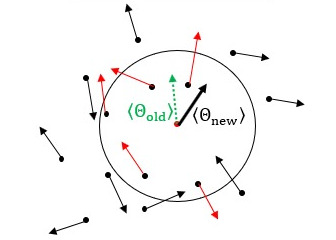
\includegraphics[width=0.3\textwidth]{images/chapter1/particle_direction.jpeg} 
	\end{figure}
\end{frame}

\begin{frame}
	\frametitle{1) Motivation and Theory}
	\textbf{Order Parameter.}
	\begin{itemize}
		\item To study phase transitions we analyse the order parameter $v_\mathrm{a}$
	
			\begin{equation}
	    		v_\mathrm{a} = \frac{1}{N v} \cdot \left| \sum_i^N \mathbf{v}^i \right| \in \left[0,1\right]
			\end{equation}
		\item Order parameter $v_\mathrm{a}$ inhibits (all) physics of the model
	\end{itemize}
\end{frame}
	\subsection{Periodic Boundaries}

\begin{frame}
	\frametitle{2) Periodic Boundaries}
	\textbf{Theory.}\footnote{\tiny{elektronik-kompendium. \url{https://www.elektronik-kompendium.de/sites/bau/0201211.htm}. Accessed on the 15.11.2021.}}
	\begin{itemize}
		\item highly doped n- and p-layer
		\item thinner barrier layer:
		    \begin{enumerate}
		        \item High field strengths due to $E = \frac{U}{d}$
		        \item At $U = U_{\text{Z}} \Rightarrow$ field kicks out electrons from crystal bonds
		        \item Avalanche-like charge multiplication
		        \item Current even in blocking direction
		    \end{enumerate}
	\end{itemize}
\end{frame}

\begin{frame}
	\frametitle{2) Periodic Boundaries}
	\textbf{Trajectory.} Example.
	\begin{itemize}
	    \item $\rho = 400, v = 0.03, R = 0.01, D_{\text{rot}} = 0.01, \Delta t = 1.0$
	    \item Representative trajectory is shown
	    \item Equilibration in $\approx 200$ steps
	\end{itemize}
	\begin{figure}[H]
  		\includegraphics[width=\textwidth]{images/chapter2/flocks_N_20_L_1.000000_v_0.030000_R_0.010000_D_0.010000.png} 
  		%\caption*{Cantillano C., Grundpraktikum 2: Halbleiterbauelemente. Internal Proceedings. University of Innsbruck , 2021.}
	\end{figure}
\end{frame}

\begin{frame}
	\frametitle{2) Periodic Boundaries}
	\textbf{Configurations.} $R$-dependence.
	\begin{itemize}
	    \item $\rho = 400, v = 0.03, D_{\text{rot}} = 0.01, \Delta t = 1.0$
	    \item Bigger $R\Rightarrow$ bigger flocks 
	\end{itemize}
	\begin{figure}[H]
  		\includegraphics[width=\textwidth]{images/chapter2/N_20_L_1.000000_v_0.030000_R_D_0.010000.png} 
  		%\caption*{Cantillano C., Grundpraktikum 2: Halbleiterbauelemente. Internal Proceedings. University of Innsbruck , 2021.}
	\end{figure}
\end{frame}

\begin{frame}
	\frametitle{2) Periodic Boundaries}
	\textbf{Phase transitions.} 2D Levels in parameter space.
	\begin{itemize}
	    \item $R$ against $\sqrt{2D_{\text{rot}}\Delta t}$
	\end{itemize}
	\begin{figure}[H]
  		
\includegraphics[width=\textwidth]{images/chapter2/r_eta_transition_2D_plots_rho_comparison.png} 
  		%\caption*{Cantillano C., Grundpraktikum 2: Halbleiterbauelemente. Internal Proceedings. University of Innsbruck , 2021.}
	\end{figure}
\end{frame}

\begin{frame}
	\frametitle{2) Periodic Boundaries}
	\textbf{Phase transitions.} 2D Levels in parameter space.
	\begin{itemize}
	    \item $\rho$ against $\sqrt{2D_{\text{rot}}\Delta t}$
	\end{itemize}
	\begin{figure}[H]
  		
\includegraphics[width=\textwidth]{images/chapter2/rho_eta_transition_2D_plots_r_comparison.png} 
  		%\caption*{Cantillano C., Grundpraktikum 2: Halbleiterbauelemente. Internal Proceedings. University of Innsbruck , 2021.}
	\end{figure}
\end{frame}

\begin{frame}
	\frametitle{2) Periodic Boundaries}
	\textbf{Phase transitions.} 2D Levels in parameter space.
	\begin{itemize}
	    \item $\rho$ against $R$
	\end{itemize}
	\begin{figure}[H]
  		
\includegraphics[width=\textwidth]{images/chapter2/rho_r_transition_2D_plots_D_comparison.png} 
  		%\caption*{Cantillano C., Grundpraktikum 2: Halbleiterbauelemente. Internal Proceedings. University of Innsbruck , 2021.}
	\end{figure}
\end{frame}
	\subsection{Reflecting Boundaries with Vision}

\begin{frame}
	\frametitle{3) Reflecting Boundaries}
	\textbf{Trajectory.} Example.
	\begin{itemize}
	    \item $\rho = 400, v = 0.03, R = 0.03, D_{\text{rot}} = 0.01, \Delta t = 1.0, N_{\text{sim}} = 1500, N_{\text{eq}} = 1000$
	    \item Representative trajectory is shown
	    \item Large fluctuations (collisions with boundary)
	\end{itemize}
	\begin{figure}[H]
  		\includegraphics[width=\textwidth]{images/chapter3/flocks_N_20_L_1.000000_v_0.030000_R_0.010000_D_0.010000.png} 
  		%\caption*{Cantillano C., Grundpraktikum 2: Halbleiterbauelemente. Internal Proceedings. University of Innsbruck , 2021.}
	\end{figure}
\end{frame}

\begin{frame}
	\frametitle{3) Reflecting Boundaries}
	\textbf{Trajectory.} Interesting Collisions.
	\begin{itemize}
	    \item $\rho = 400, v = 0.03,  R = 0.03, D_{\text{rot}} = 0.01, \Delta t = 1.0, N_{\text{sim}} = 1500, N_{\text{eq}} = 1000$
	    \item Two incoming flocks $\rightarrow$ one outgoing flock 
	\end{itemize}
	\begin{figure}[H]
  		\includegraphics[width=\textwidth]{images/chapter3/collision_N_20_L_1.000000_v_0.030000_R_0.030000_D_0.010000.png} 
  		%\caption*{Cantillano C., Grundpraktikum 2: Halbleiterbauelemente. Internal Proceedings. University of Innsbruck , 2021.}
	\end{figure}
\end{frame}

\begin{frame}
	\frametitle{3) Reflecting Boundaries}
	\textbf{Configurations.} $R$-dependence.
	\begin{itemize}
	    \item $\rho = 400, v = 0.03, D_{\text{rot}} = 0.01, \Delta t = 1.0, N_{\text{sim}} = 1500, N_{\text{eq}} = 1000$
	    \item Bigger $R\Rightarrow$ bigger flocks 
	    \item Flocking stronger compared to periodic boundaries
	\end{itemize}
	\begin{figure}[H]
  		\includegraphics[width=\textwidth]{images/chapter3/N_20_L_1.000000_v_0.030000_R_D_0.010000_rbc.png} 
  		%\caption*{Cantillano C., Grundpraktikum 2: Halbleiterbauelemente. Internal Proceedings. University of Innsbruck , 2021.}
	\end{figure}
\end{frame}

\begin{frame}
	\frametitle{3) Reflecting Boundaries}
	\textbf{Phase transitions.} 2D Levels in parameter space.
	\begin{itemize}
	    \item $R$ against $\sqrt{2D_{\text{rot}}\Delta t}$
	\end{itemize}
	\begin{figure}[H]
  		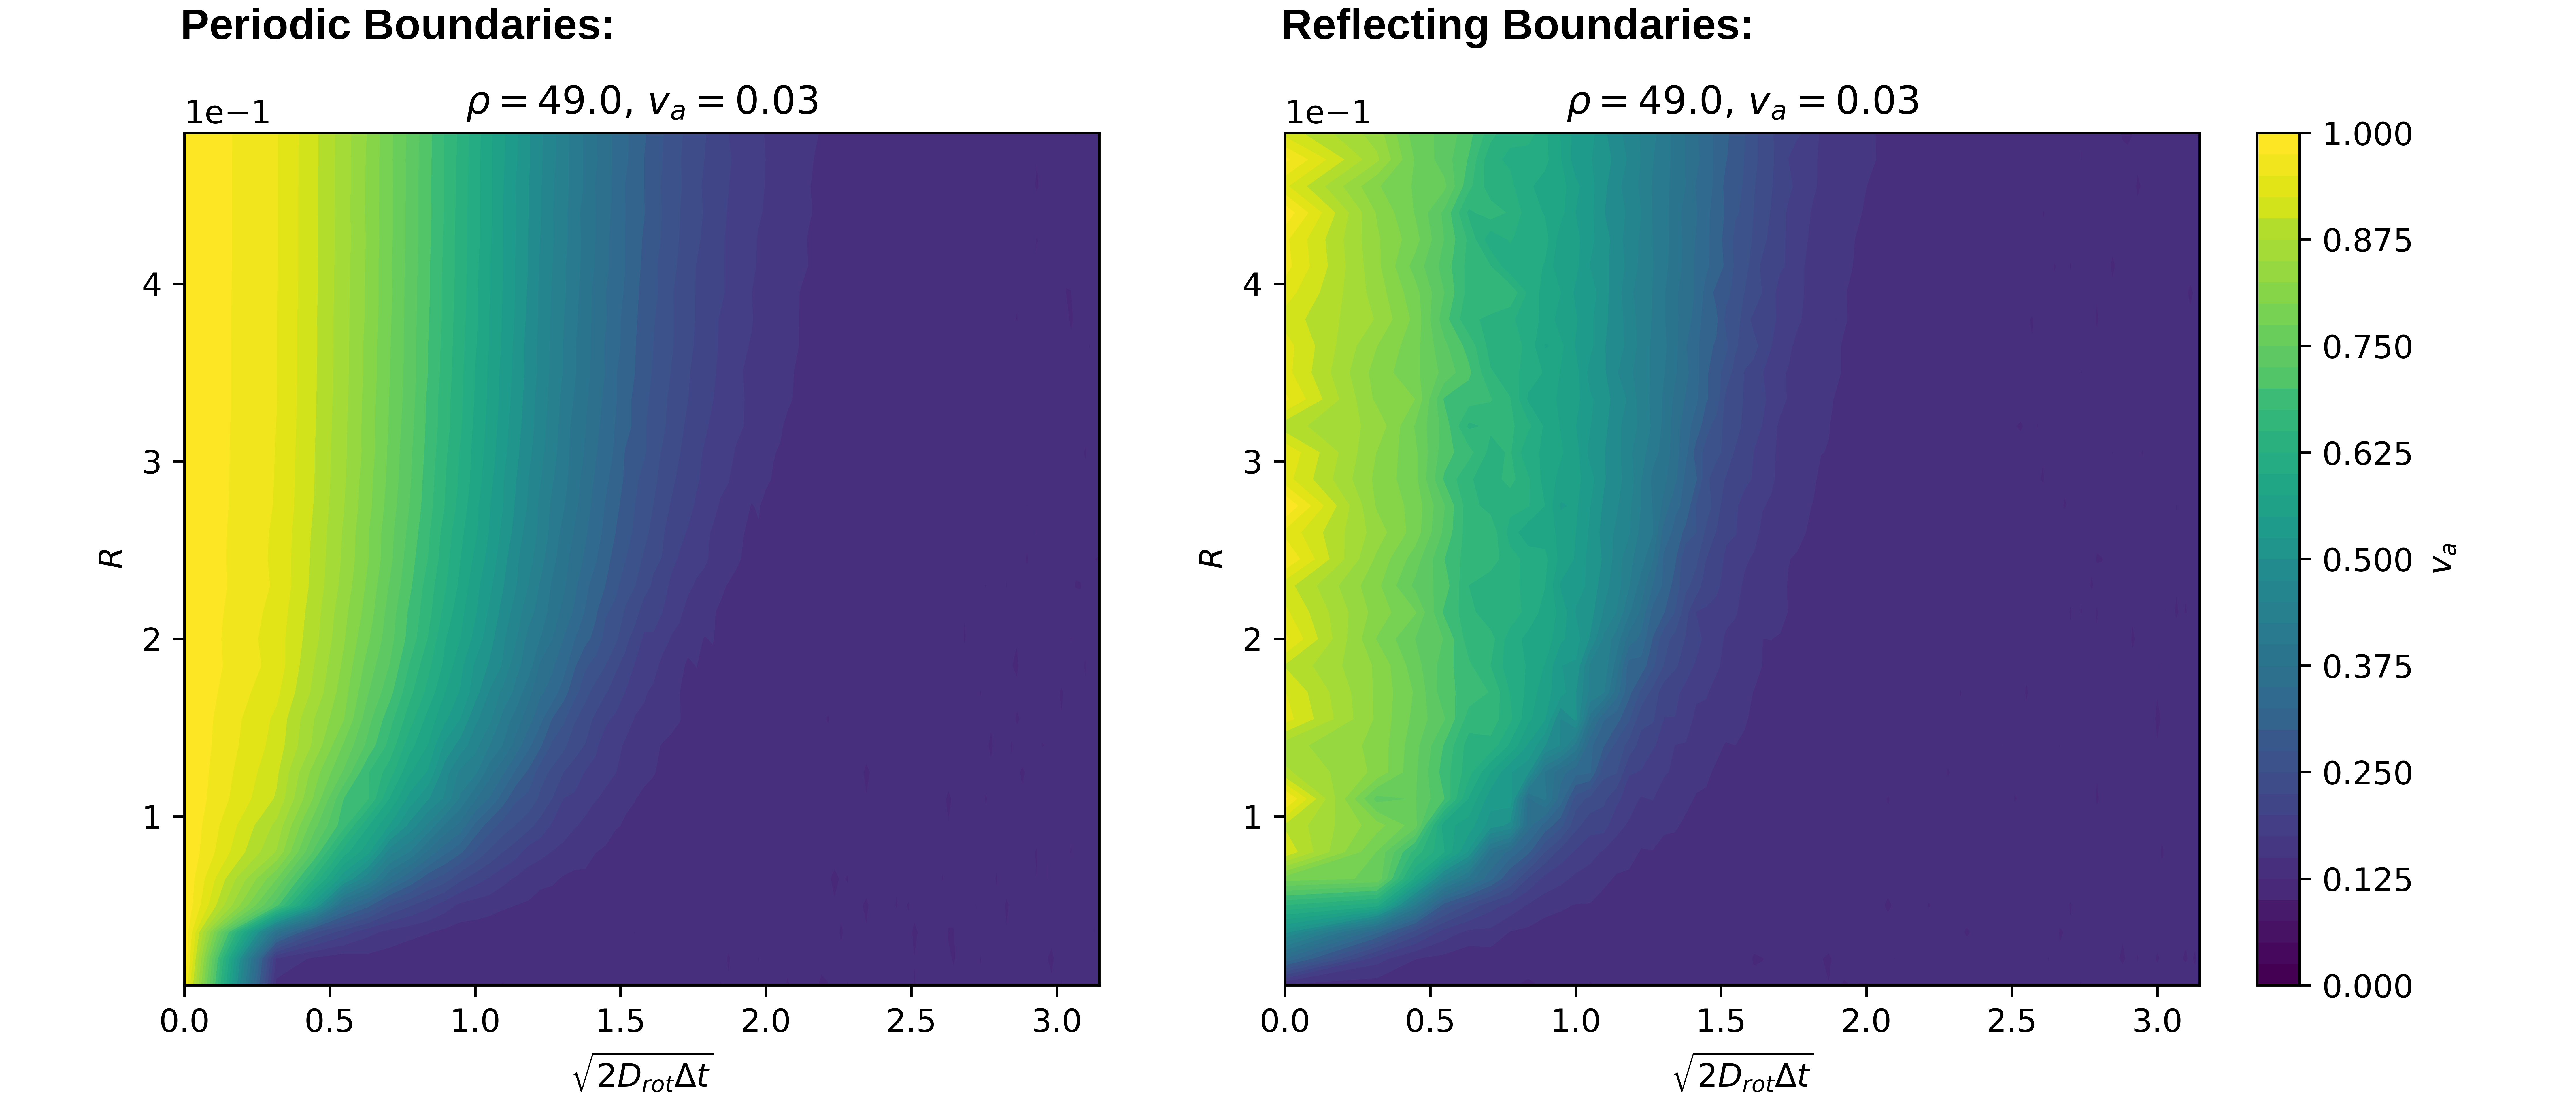
\includegraphics[width=0.9\textwidth]{images/chapter3/r_eta_transition_2D_comparison_pbc_rbc.png} 
  		%\caption*{Cantillano C., Grundpraktikum 2: Halbleiterbauelemente. Internal Proceedings. University of Innsbruck , 2021.}
	\end{figure}
\end{frame}

\begin{frame}
	\frametitle{3) Reflecting Boundaries}
	\textbf{Phase transitions.} 2D Levels in parameter space.
	\begin{itemize}
	    \item $\rho$ against $\sqrt{2D_{\text{rot}}\Delta t}$
	\end{itemize}
	\begin{figure}[H]
  		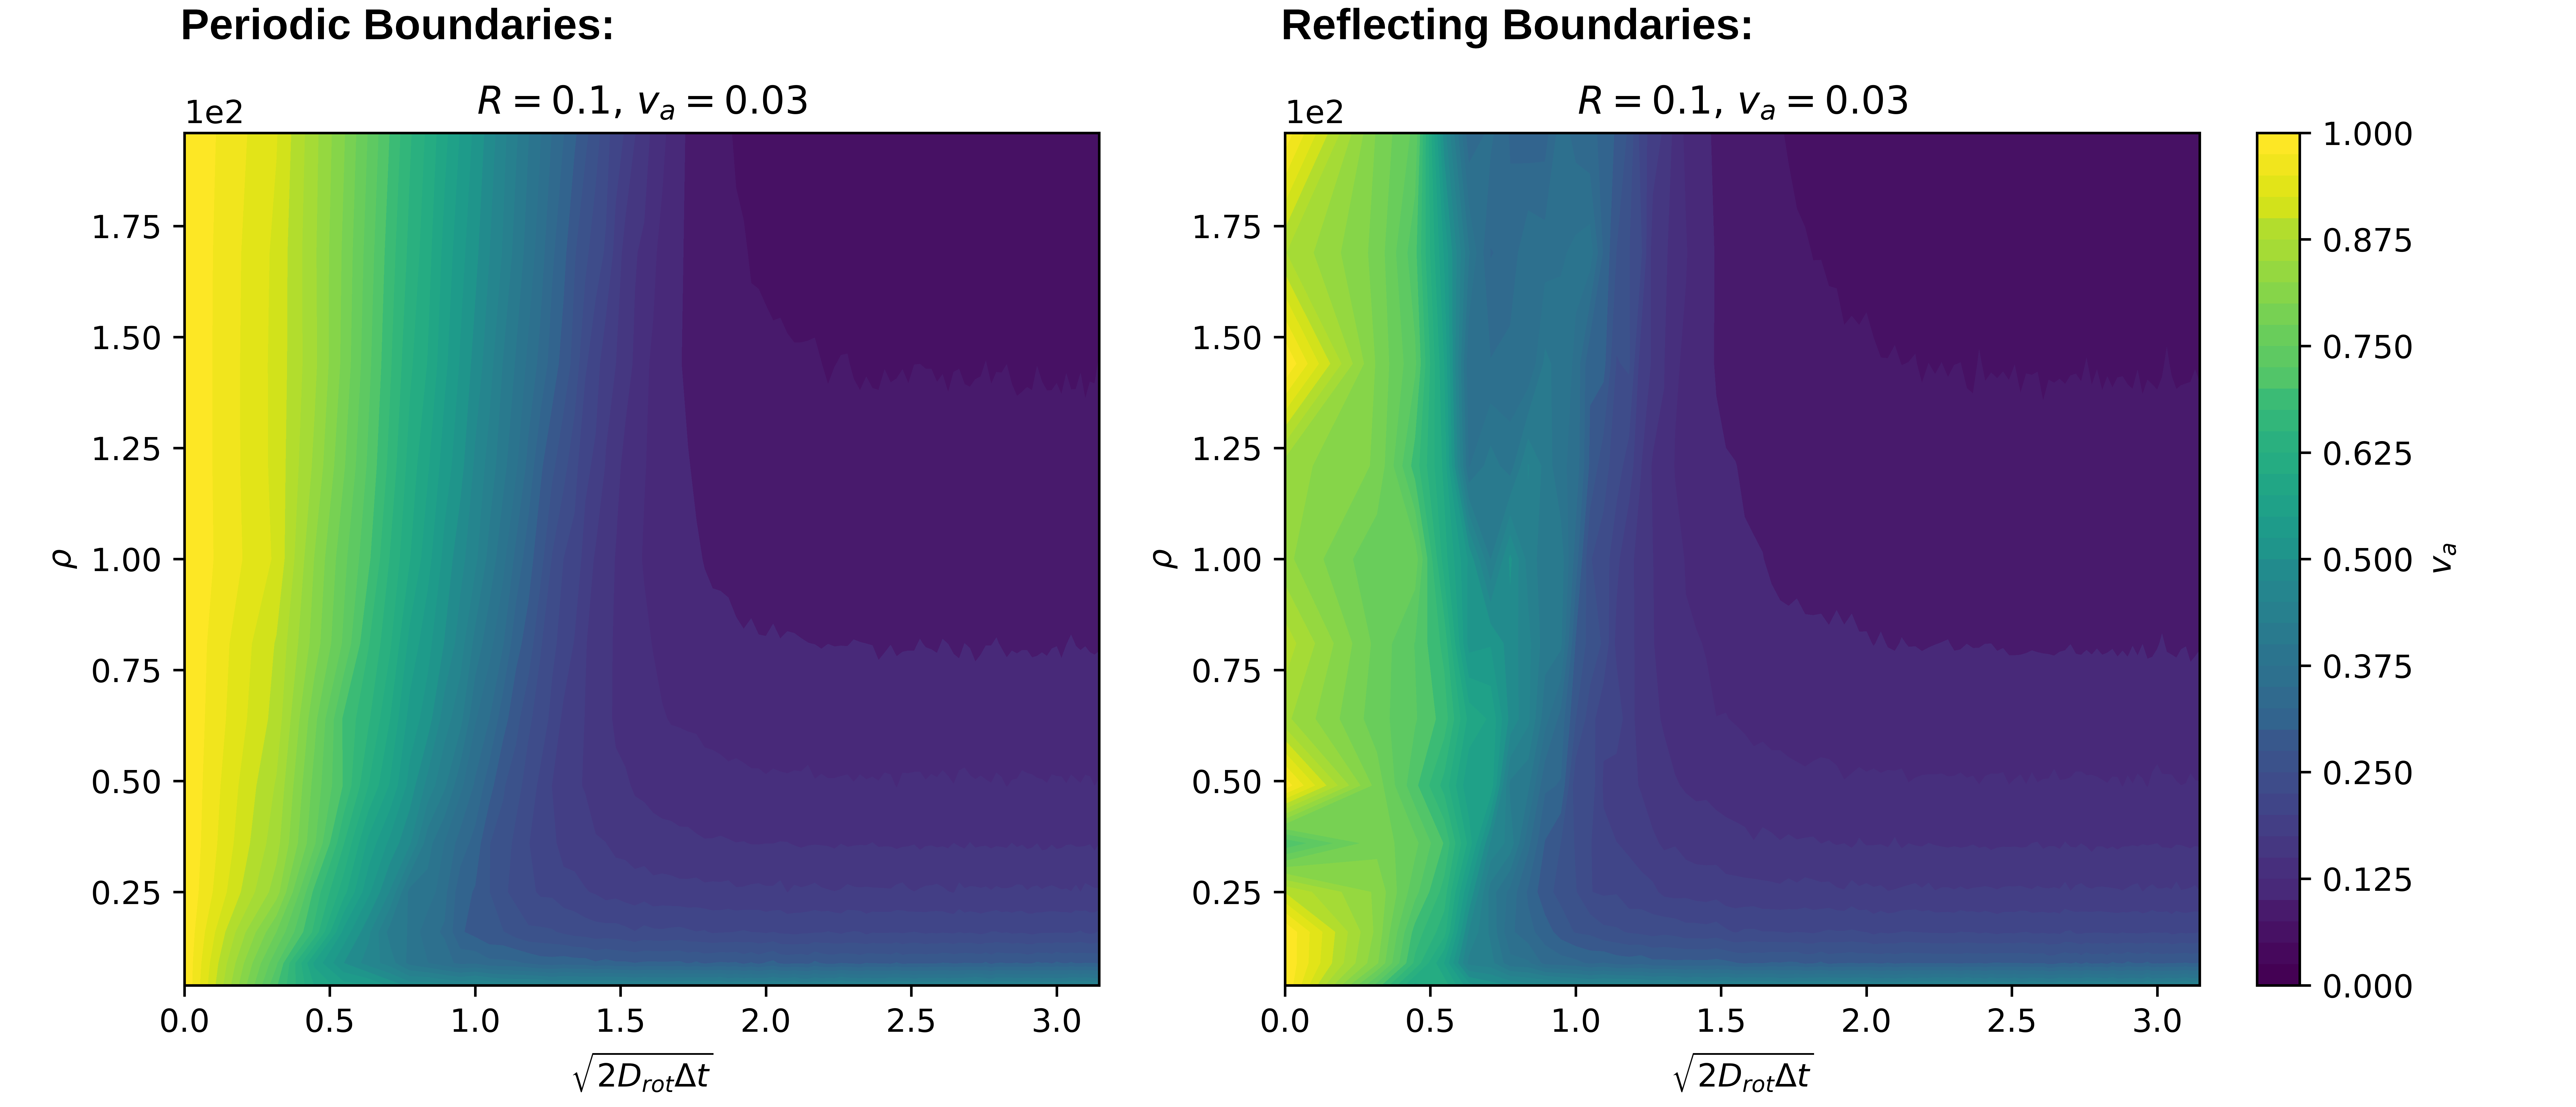
\includegraphics[width=0.9\textwidth]{images/chapter3/rho_eta_transition_2D_comparison_pbc_rbc.png} 
  		%\caption*{Cantillano C., Grundpraktikum 2: Halbleiterbauelemente. Internal Proceedings. University of Innsbruck , 2021.}
	\end{figure}
\end{frame}
	\subsection{Reflecting Boundaries}

\begin{frame}
	\frametitle{4) Periodic Boundaries with Vision}
	\textbf{Implementation.}
	\begin{itemize}
	    \item Just particles in circle segment defined by vision angle $\varphi$ are considered
	\end{itemize}
	\begin{figure}[H]
  		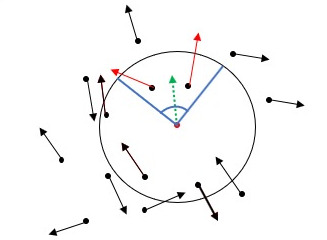
\includegraphics[width=0.4\textwidth]{images/chapter4/particle_vision.jpeg} 
	\end{figure}
\end{frame}

\begin{frame}
	\frametitle{4) Periodic Boundaries with Vision}
	\textbf{Trajectory.} Comparing Angles.
	\begin{itemize}
	    \item $\rho = 400, v = 0.03, R = 0.03, D_{\text{rot}} = 0.01, \Delta t = 1.0$
	    \item $v_a$ grows with vision angle
	\end{itemize}
	\begin{figure}[H]
  		\includegraphics[width=\textwidth]{images/chapter4/trajectory_comp_N_20_L_1.000000_v_0.030000_R_0.030000_D_0.010000.png} 
  		%\caption*{Cantillano C., Grundpraktikum 2: Halbleiterbauelemente. Internal Proceedings. University of Innsbruck , 2021.}
	\end{figure}
\end{frame}

\begin{frame}
	\frametitle{4) Periodic Boundaries with Vision}
	\textbf{Configurations.} Comparing Angles.
	\begin{itemize}
	    \item $\rho = 400, v = 0.03, R = 0.03, D_{\text{rot}} = 0.01, \Delta t = 1.0$
	    \item Flock size grows with vision angle
	\end{itemize}
	\begin{figure}[H]
  		\includegraphics[width=\textwidth]{images/chapter4/configuration_comp_N_20_L_1.000000_v_0.030000_R_0.030000_D_0.010000.png} 
  		%\caption*{Cantillano C., Grundpraktikum 2: Halbleiterbauelemente. Internal Proceedings. University of Innsbruck , 2021.}
	\end{figure}
\end{frame}

\begin{frame}
	\frametitle{4) Periodic Boundaries with Vision}
	\textbf{Phase transitions.} 2D Levels in parameter space.
	\begin{itemize}
	    \item $R$ against $\sqrt{2D_{\text{rot}}\Delta t}$
	    \item Region of ordered phase increases with vision angle
	\end{itemize}
	\begin{figure}[H]
  		
\includegraphics[width=0.9\textwidth]{images/chapter4/phase_comp_N_20_L_1.000000_v_0.030000_R_0.030000_D_0.010000.png} 
  		%\caption*{Cantillano C., Grundpraktikum 2: Halbleiterbauelemente. Internal Proceedings. University of Innsbruck , 2021.}
	\end{figure}
\end{frame}




	\subsection{Reflecting Boundaries with Vision}

\begin{frame}
	\frametitle{5) Reflecting Boundaries with Vision.}
	\textbf{Theory.} Symbol.
	\begin{figure}[H]
  		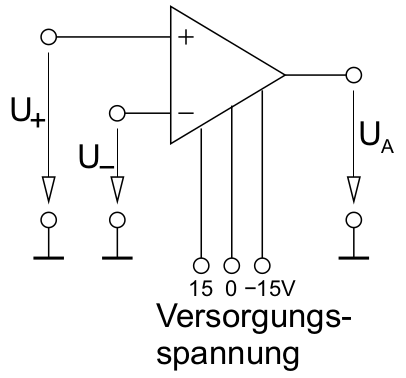
\includegraphics[width=0.3\textwidth]{images/chapter5/8_theory_scheme_operational_amplifier.png} 
  		\caption*{Cantillano C., Grundpraktikum 2: Halbleiterbauelemente. Internal Proceedings. University of Innsbruck , 2021.}
	\end{figure}
\end{frame}
	\subsection{Conclusion}

\begin{frame}
	\frametitle{6) Conclusion}
	\textbf{Summary.}
	\begin{itemize}
	    \item Successful implementation of the 2D Vicsek model
	    \item Demonstration of flocking behaviour
	    \item Analysis of phases and their dependence on controlling parameters 
	    	\begin{itemize}
	    		\item Results of \textit{Vicsek et al.} have been reproduced
	    	\end{itemize}
	    \item Implementation of reflecting boundaries
	    	\begin{itemize}
	    		\item Slight influence on phase transitions
	    		\item Larger fluctuations of $v_a$
	    	\end{itemize}
	    \item Implementation of vision
	\end{itemize}
\end{frame}

\begin{frame}
	\frametitle{6) Conclusion}
	\textbf{Outlook.}
	\begin{itemize}
	    \item Investigate other order parameters? e. g. average size of flocks
	    \item Investigate dependence on $v$
	    \item Also update $v$ in every time step
	    \item Optimize simulation for higher particle numbers/densities
	    \item Higher dimensions
	\end{itemize}
\end{frame}
		
	%% to show a last slide similar to the title slide: information for the last page
	\title{Thank you for your attention!}
	\subtitle{}
	\section{End}
	
	\appendix
	\begin{frame}
		\frametitle{A-2) Periodic Boundaries}
		\textbf{Phase transitions.} 2D Levels in parameter space.
		\begin{itemize}
	    	\item $\rho$ against $R$
		\end{itemize}
		\begin{figure}[H]
  			
\includegraphics[width=\textwidth]{images/chapter2/rho_r_transition_2D_plots_D_comparison.png} 
  		%\caption*{Cantillano C., Grundpraktikum 2: Halbleiterbauelemente. Internal Proceedings. University of Innsbruck , 2021.}
		\end{figure}
	\end{frame}
	
	\begin{frame}
		\frametitle{A-3) Reflecting Boundaries}
		\textbf{Phase transitions.} Example for critical exponent.
		\begin{itemize}
	    	\item $v_a \approx \left(\sqrt{2D_{\text{rot}}^c\Delta t} - \sqrt{2D_{\text{rot}}\Delta t}\right)^{\beta}$
	    	\item Here: $\sqrt{2D_{\text{rot}}^c\Delta t} \approx 1.7$ (see figure on the left)
	    	\item Linear fit: slope $=\num{1.1(3)}$, offset $=\num{1.0(1)} \Rightarrow \beta = \num{1.1(3)}$???
		\end{itemize}
		\begin{figure}[H]
  			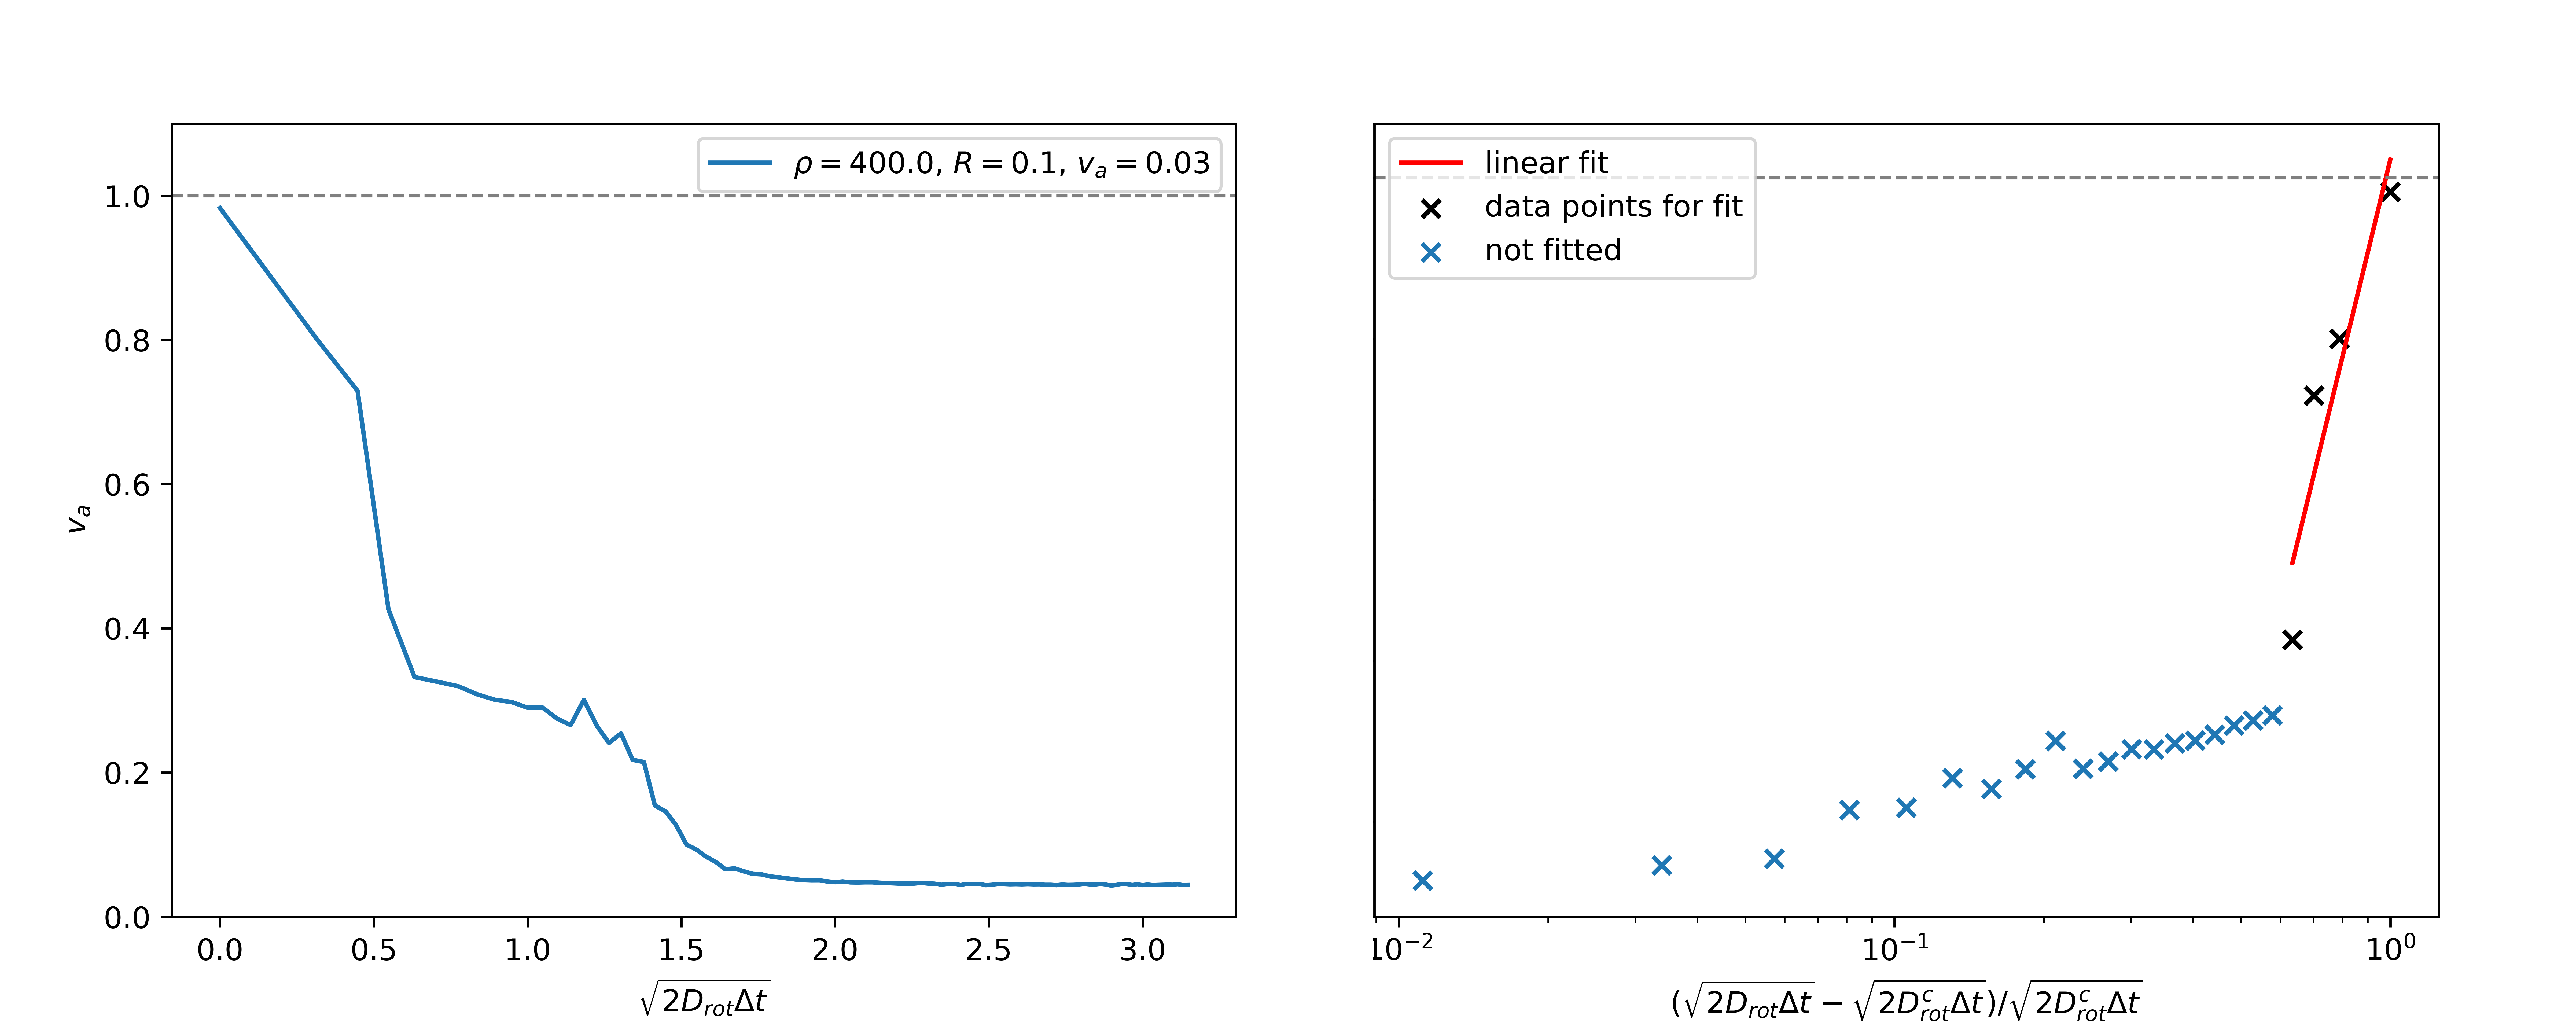
\includegraphics[width=0.8\textwidth]{images/chapter3/rbc_critial_exponent_gone_wrong.png} 
  			%\caption*{(right) Tamás Vicsek, András Czirók, Eshel Ben-Jacob, Inon Cohen, and Ofer Shochet. Novel Type of Phase Transition in a System of Self-Driven Particles. Phys. Rev. Lett. 75, 1226 – Published 7 August 1995}
		\end{figure}
\end{frame}
	
	\begin{frame}
		\frametitle{A-5) Reflecting Boundaries with Vision}
		\textbf{Trajectories.} Dependence on Vision Angle .
		\begin{itemize}
	    	\item $\rho = 400, v = 0.03, R = 0.025, D_{\text{rot}} = 0.01, \Delta t = 1.0, N_{\text{sim}} = 1500, N_{\text{eq}} = 1000$
	    	\item $v_a$ grows with vision angle
	    	\item Less order and higher fluctuations for rbc
		\end{itemize}
		\begin{figure}[H]
  			\includegraphics[width=\textwidth]{images/chapter5/trajectory_comp_N_20_L_1.000000_v_0.030000_R_0.030000_D_0.010000.png} 
  		%\caption*{Cantillano C., Grundpraktikum 2: Halbleiterbauelemente. Internal Proceedings. University of Innsbruck , 2021.}
		\end{figure}
	\end{frame}
\end{document}

